\chapter{Evoluindo uma plataforma de rede social}
\label{evol-rede-social}

Neste capítulo é discutida a plataforma Noosfero, desde sua arquitetura até os processos de desenvolvimento da comunidade. Além disso, é apresentado o Comunidade.UnB, rede de colaboração livre, no qual são propostas evoluções para que se torne um ambiente híbrido utilizado por professores e alunos.

\section{Noosfero}
\label{noosfero}

O Noosfero \footnote{Disponível em: \url{http://www.noosfero.org}} é uma plataforma livre para criação de redes sociais, desenvolvida em 2007, pela Cooperativa de Tecnologias Livres - Colivre \footnote{Disponível em: \url{http://www.colivre.coop.br}}, sob a licença AGPL\footnote{Licença de software GNU} V3, com a proposta de facilitar a criação de redes sociais personalizadas, livres e autônomas e a geração de conteúdo colaborativo.

Além das funcionalidades de rede social, com foco na produção e compartilhamento de conteúdo, o Noosfero permite que dentro da rede cada usuário e comunidade tenha o seu espaço com total flexibilidade de personalização visual e gerenciamento de conteúdo. São exemplos de portais que utilizam o Noosfero: o Participa BR \footnote{Disponível em: \url{https://www.participa.br/}}, Stoa\footnote{Disponível em: \url{http://stoa.usp.br/}}, Portal da FGA\footnote{Disponível em: \url{http://fga.unb.br/}} e o novo Portal do Software público Brasileiro \footnote{Disponível em: \url{https://portal.softwarepublico.gov.br/}}.

O Noosfero foi desenvolvido na linguagem de programação Ruby, atualmente na versão 2.2.0, e utiliza o \textit{framework} aplicações web \textit{Ruby on Rails} \footnote{Disponível em: \url{http://rubyonrails.org/}}, versão 3.2.21. E utiliza também padrões arquiteturais de software Model-View-Controller (MVC), e o padrão de plugins que serão apresentados na seção \ref{arquitetura}.

A escolha da linguagem \textit{Ruby} foi decisiva no Noosfero, pois possui uma sintaxe simples, que facilita a manutenibilidade do sistema, característica importante em projetos de software livre que tendem a atrair colaboradores externos \cite{meirelles2013}. A escolha do \textit{Rails} foi influenciada pelos seus conceitos básicos que auxiliam em sua produtividade: ``Não Repita a Si Mesmo'' (DRY-\textit{Don't Repeat Yourself}) e ``convenção sobre configuração'' (\textit{Convention Over Configuration}) \cite{akita2006repensando}. Além disso , por questões de segurança, o Noosfero é homologado para a versão \textit{stable} do \textit{Debian}, acompanhando a versão do \textit{Ruby} e do \textit{Rails} dessa distro.

\subsection{Práticas de desenvolvimento da comunidade Noosfero}
\label{proc-desenvol-comunidade}
% - ciclos
% - repositorio
% - commiters/revisao
% - testes

Para que novos desenvolvedores colaborem com o Noosfero, a comunidade utiliza em seu próprio \textit{site} uma seção para o desenvolvimento. Nessa seção, encontram-se os manuais com os passos para instalação do ambiente, descrição dos \textit{plugins} disponíveis, instruções para a personalização da plataforma através de temas além de informações arquiteturais da plataforma. Para realizar o controle de itens a fazer, como a implementação de novas funcionalidades ou correção de bugs é utilizado um \textit{Issue Tracker} do repositório oficial no GitLab \footnote{Disponível em: \url{https://gitlab.com/noosfero/noosfero}}.

Uma vez que o desenvolvedor ou usuário tenha registro no GitLab, é possível utilizar o \textit{Issue Tracker} para cadastrar novas funcionalidades ou \textit{bugs} de maneira simples seguindo os seguintes passos:

\begin{enumerate}
\item preencher o campo título;
\item definir a descrição do item, se existir, é necessário especificar com qual \textit{plugin} o item está relacionado;
\item associar um desenvolvedor responsável pela sua implementação \textit{issue};
\item definir as \textit{labels} da funcionalidade, onde é especificado ao que está relacionado a nova \textit{issue}.
\end{enumerate}

Após a criação da \textit{issue}, todos os membros da comunidade podem visualizar os dados e especificações, bem como discutir sobre os propósitos e formas de implementação da funcionalidade.

A Figura \ref{issue-tracker} evidencia o \textit{Issue Tracker} do Noosfero onde é possível verificar os itens que foram mapeados e seus respectivos \textit{status}, se ainda estão abertas ou fechadas, além de um filtro para os autores e os marcadores envolvidos à cada uma delas. Dessa forma, é possível priorizar os itens identificados como sendo de maior importância para os usuários e desenvolvedores.

\begin{figure}[h]
    \centering
    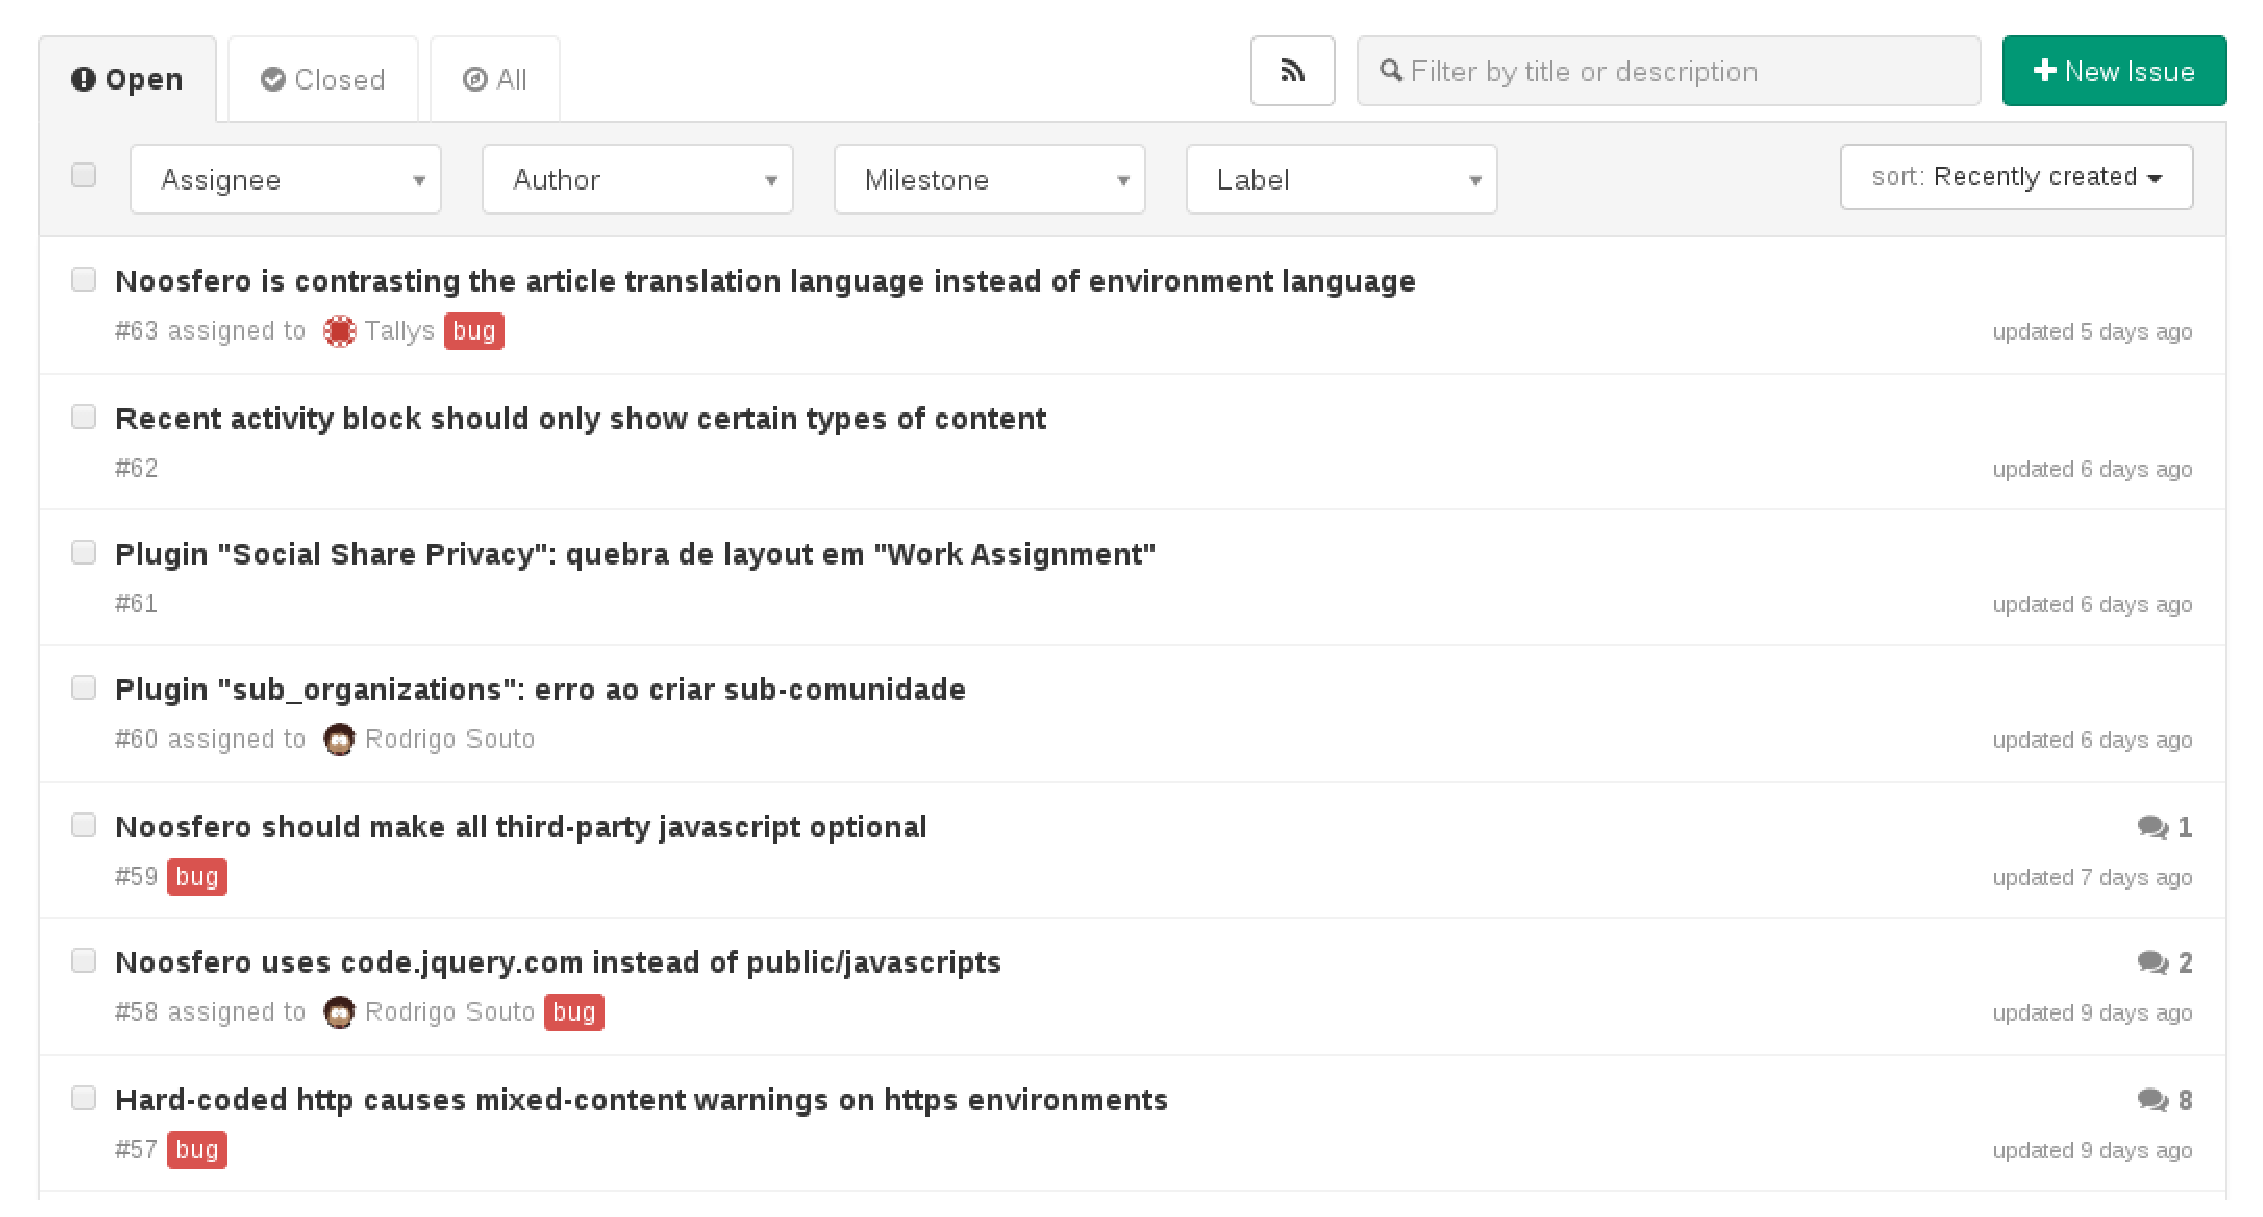
\includegraphics[keepaspectratio=true,scale=0.4]
      {figuras/issueTrackerGitLab.eps}
    \caption{Issue Tracker no GitLab}
    \label{issue-tracker}
\end{figure}

Priorizando a comunicação entre os desenvolvedores, a comunidade compartilha canais \footnote{Canais do Noosfero: \textit{\#noosfero-br} e \textit{\#noosfero}} de comunicação pelo IRC (\textit{Internet Relay Chat}). Nesses os desenvolvedores podem compartilhar conhecimento e realizarem discussões técnicas sobre as implementações.

A implementação é realizada pelo desenvolvedor que tem a responsabilidade de manter a qualidade do código produzido bem como realizar todos os testes relacionados à funcionalidade implementada. Uma vez que este primeiro passo esteja concluído o código é submetido a um \textit{merge-request} onde um dos desenvolvedores do \textit{core} efetua a revisão para verificar se está de acordo com os padrões esperados, e aprova ou não, a inclusão do código na \textit{branch} principal do Noosfero.

A comunidade Noosfero recomenda práticas de desenvolvimento como o TDD, \textit{Test Driven Development} ou Desenvolvimento orientado a testes), combinado com o BDD \footnote{\url{https://cukes.info/}} (\textit{Behavior Driven Development}) ou Desenvolvimento Guiado por Comportamento, que auxiliar o desenvolvedor a criar testes e integrar regras de negócio com a linguagem de programação, mantendo o foco no comportamento do software \cite{north2006introducing}.

Para realizar o controle de versão e gerenciamento do código fonte é utilizado o \textit{Git}, uma ferramenta livre de versionamento distribuído de código fonte. O repositório oficial do Noosfero encontra-se no software livre Gitlab com um espelho no Github\footnote{\url{https://github.com/noosfero/noosfero}}. Na página de desenvolvimento da comunidade existe uma série de recomendações sobre o envio de \textit{patches} para o Noosfero, incluindo como versionamentos e solicitações de inclusão de seu \textit{patch}, ou \textit{merge-request}.

\subsection{Arquitetura}
\label{arquitetura}

Para a evolução de um software de forma adequada é importante o conhecimento da arquitetura do sistema, para não comprometer todo o planejamento realizado na concepção do projeto. Desse modo conhecer e entender a arquitetura de funcionamento do Noosfero é uma etapa fundamental para o densevolvimento de novas funcionalidades para a plataforma.

\begin{figure}[h]
    \centering
    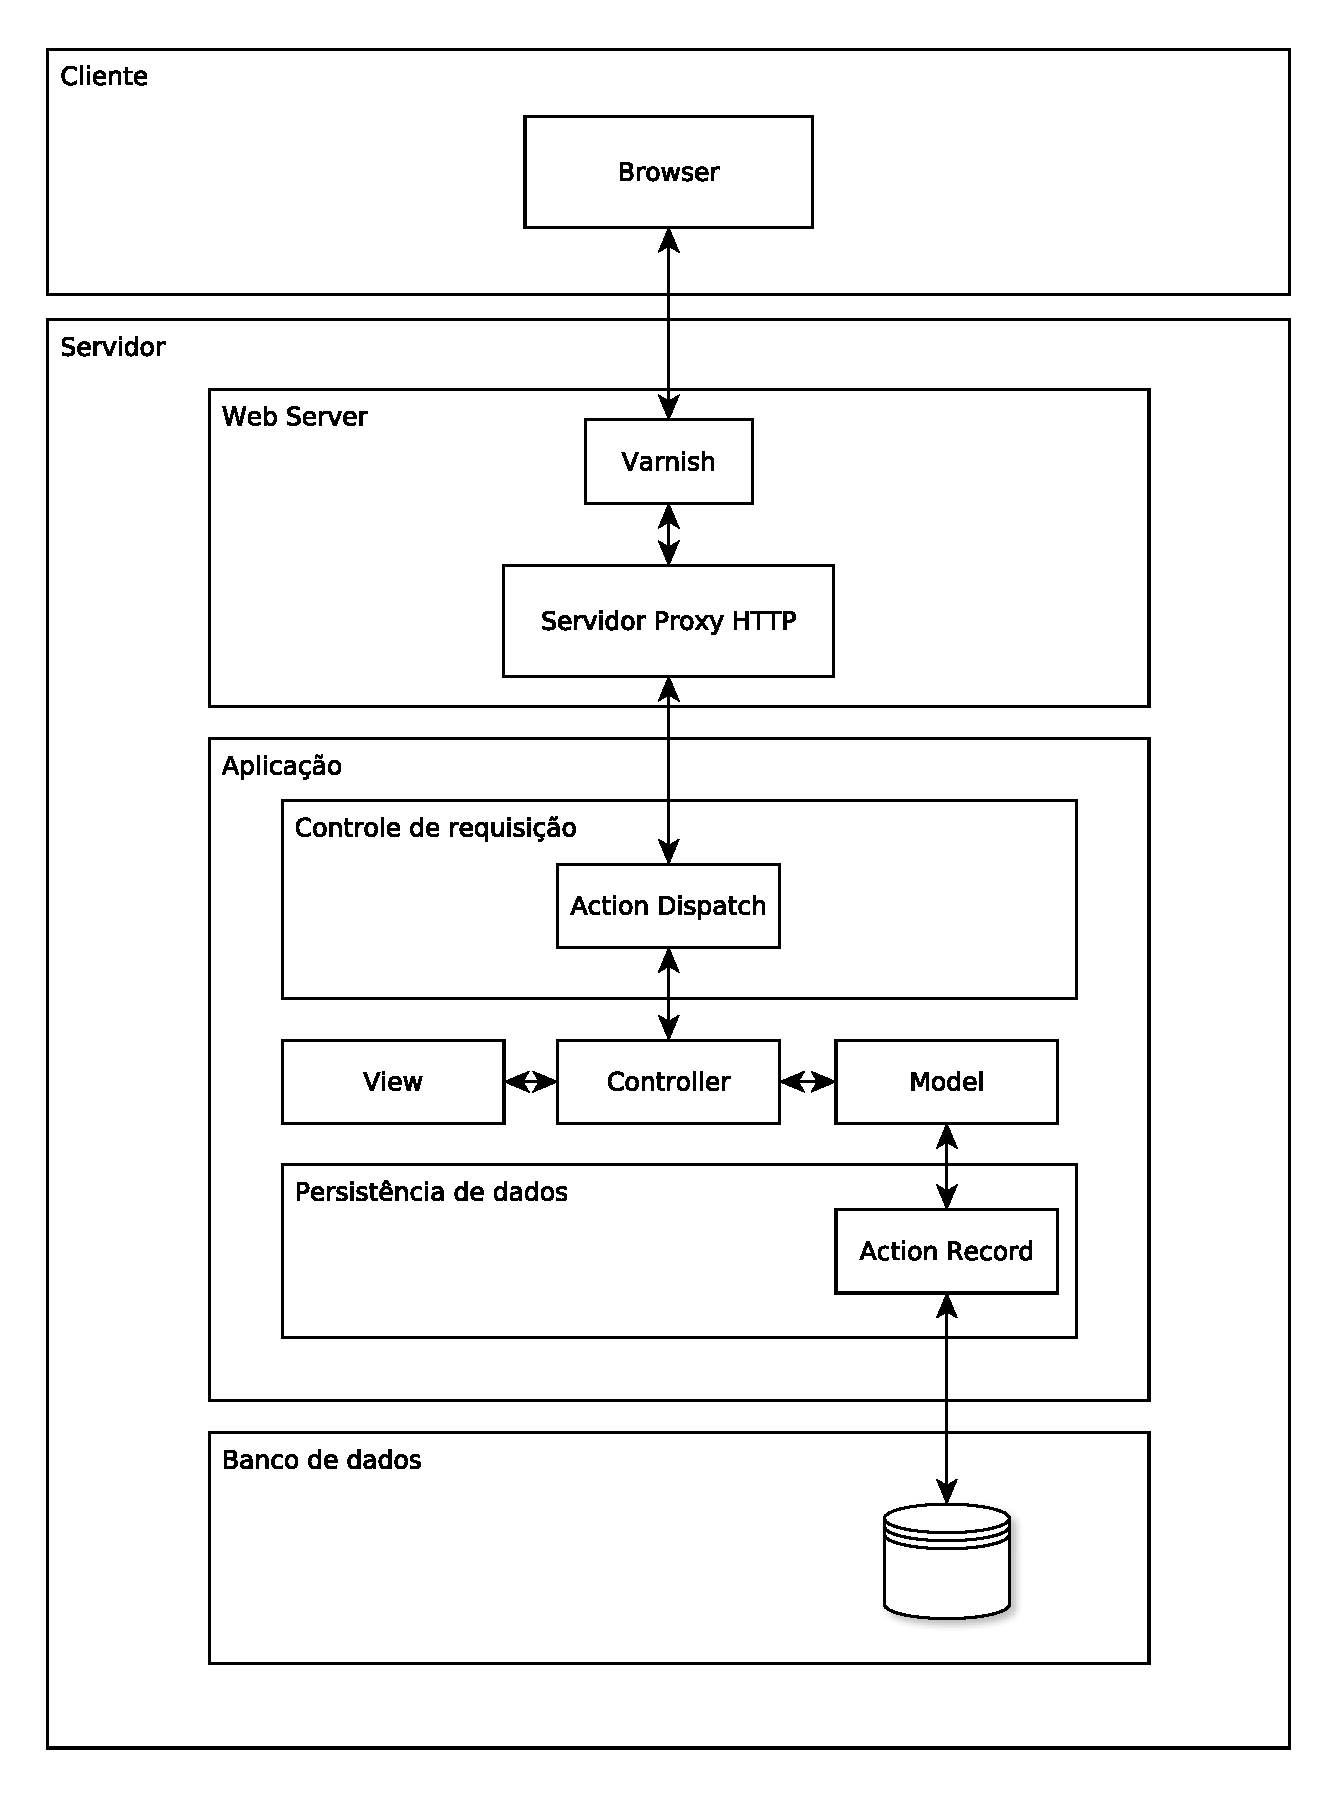
\includegraphics[keepaspectratio=true,scale=0.4]
      {figuras/DiagramaDeArquitetura.eps}
    \caption{Arquitetura do Noosfero}
    \label{arquitetura-noosfero}
\end{figure}

A Figura \ref{arquitetura-noosfero} apresenta uma visão de alto nível da arquitetura do Noofero. Basicamente tem-se uma arquitetura cliente-servidor onde o cliente via \textbf{\textit{Browser}} solicita um conteúdo ou uma função para o servidor Noosfero, que aguarda requisições de entrada para processá-las e compartilhar recursos com o cliente.

Do lado do servidor, temos basicamente três camadas de abstração: \textit{Web-Server}, \textit{aplicação} e \textit{Banco de dados}. Na primeira camada temos dois componentes responsáveis por processar e acelerar todas as requisições de entrada e saída:

\begin{itemize}
\item Varnish: é um acelerador para sites web dinâmicos com alto volume de conteúdo que utiliza \textit{proxy} HTTP Reverso. Sua efiência deve-se ao fato dele armazenar o conteúdo HTTP requisitado na memória RAM, fazendo com que o servidor não consulte e processe diversas vezes o mesmo conteúdo solicitado.
\item Servidor Proxy HTTP: pode ser utilizado o Apache ou Nginx \footnote{\url{http://nginx.org}} que ajudam a melhorar o desempenho funcionando como um servidor proxy HTTP reverso que processa as requisições de entrada e saída e as encaminha para a aplicação executá-las.
\end{itemize}

Na camada da aplicação, foi considerada uma camada responsável pelo controle de requisições, que é efetuada pelo componente \textbf{\textit{Action Dispatch}}, que lida com o mapeamento de todas as requisições, \textit{cookies} e sessão para suas respectivas \textit{controllers}.

Na aplicação, utiliza-se o padrão de arquitetura de software MVC\footnote{Model-view-controller} onde a \textbf{\textit{controller}} controla o fluxo da aplicação,relacionando as entidades de \textit{model} e de \textit{view} através de chamadas de métodos. A \textbf{\textit{model}} representa as entidades do domínio da aplicação, onde a lógica do sistema são implementadas. A \textbf{\textit{view}} é a interface de comunicação com o usuário, ou seja as páginas HTML apresentadas no navegador.

Ainda na camada da aplicação tem-se o \textbf{\textit{Active Record}} que é um ORM \footnote{object-relational mapping}, um mapeador entre objetos e registros de uma tabela, onde cada classe de modelo possui uma tabela correspondente à ela no banco de dados.

Por fim temos a camada de banco de dados que recebe requisições da camada de persistência de dados e por meio de um sistema gerenciador de banco de dados (SGBD) realizam operações na base de dados.

\subsection{Modelo de domínio}

Para \citeonline[p. 160]{larman2002utilizando}, um modelo de domínio é a representação visual de classes conceituais ou objetos do mundo real em um domínio, que também podem ser chamados de modelos conceituais, modelos de objetos de domínio e modelos de objetos de análise. Dessa forma, é necessário o seu entendimento para realizar a evolução da plataforma.

\begin{figure}[h]
    \centering
    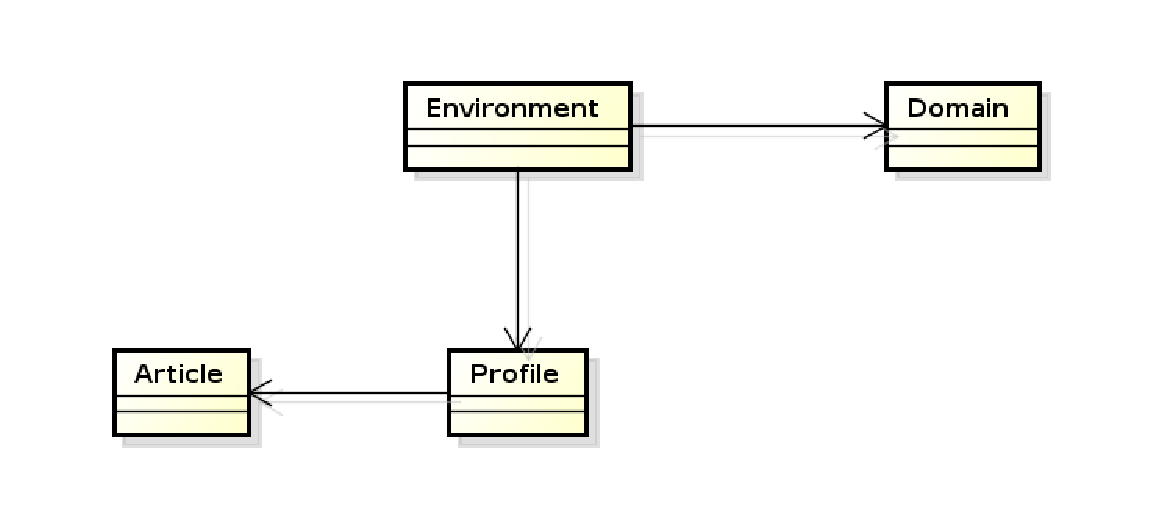
\includegraphics[keepaspectratio=true,scale=0.65]
      {figuras/domain_main.eps}
    \caption{Relações entre entidades de domínio ambiente, domínio e perfis. Extraído de: \cite{bucher2013rede}}
    \label{domain_main}
\end{figure}

O Noosfero é uma plataforma que tem suporte a vários ambientes de rede social dentro de uma mesma instalação. A Figura \ref{domain_main} mostra-se o funcionamento geral do Noosfero com suas quatro principais classes \textbf{\textit{Domain}}, \textbf{\textit{Environment}}, \textbf{\textit{Profile}} e \textbf{\textit{Article}} (Em português: Domínio, Ambiente, Perfil e Artigo respectivamente). Analisando o modelo verifica-se que na implementação é necessário que exista pelo um domínio e partir disso é possível criar várias instâncias de Ambiente na aplicação.

\begin{figure}[h]
    \centering
    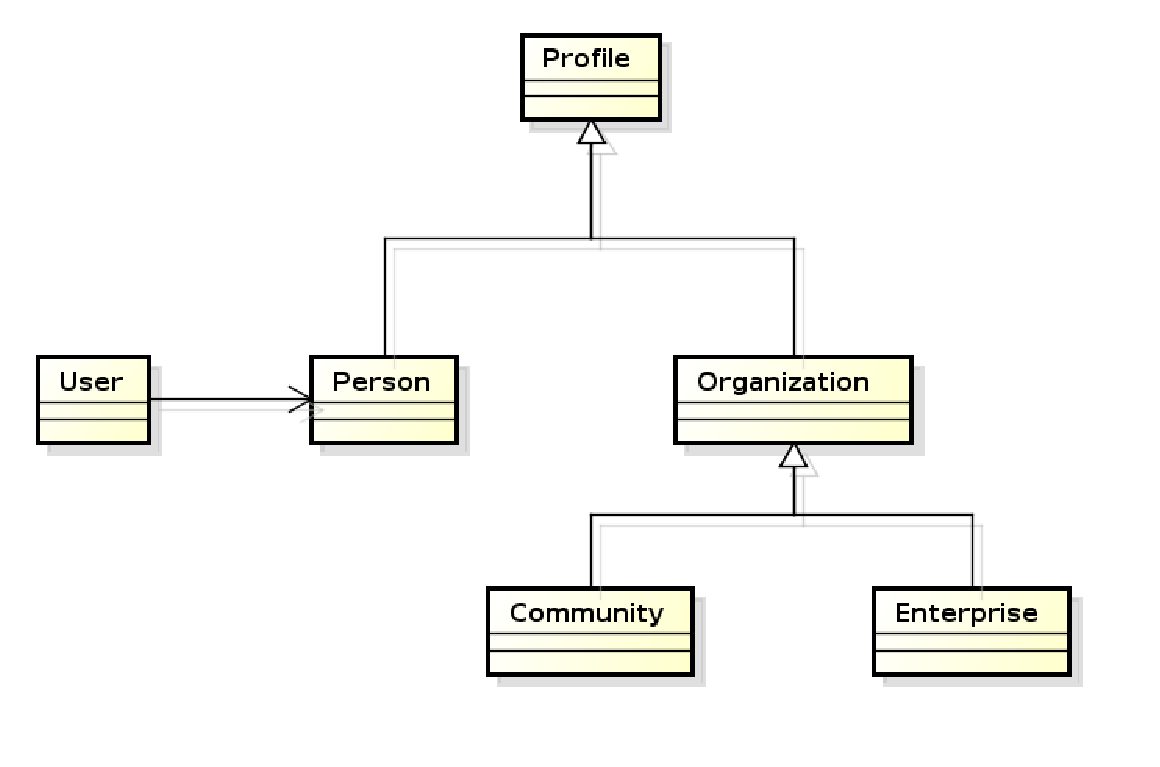
\includegraphics[keepaspectratio=true,scale=0.6]
      {figuras/domain_profiles.eps}
    \caption{Entidades de domínio: tipos de perfis. Extraído de: \cite{bucher2013rede}}
    \label{domain_profiles}
\end{figure}

A entidade Profile é uma generalização das entidades \textbf{\textit{Person}} (Pessoa) e \textbf{\textit{Organization}} (Organização), como pode ser visto na Figura \ref{domain_profiles}. Nesse mesmo modelo percebe-se que Organization é especializada nas entidades concretas \textbf{\textit{Community}} (Comunidade e Enterprise (Empreendimento). A herança é um mecanismo pelo qual qual uma classe sub-classe pode estender uma super-classe, onde basicamente isola-se métodos ou atributos em comum dentro de uma classe pai (super-classe), enquanto as especialidades são responsabilidade das classes filhas (sub-classe).

Por questões de design do código da aplicação foi criada uma entidade \textbf{\textit{User}}, ou Usuário, que é mantida separada da entidade Pessoa, que é quem implementa a lógica de autenticação da aplicação. Desta forma a lógica de autenticação fica separada da lógica de visualização e personalização do perfil.

\begin{figure}[h]
    \centering
    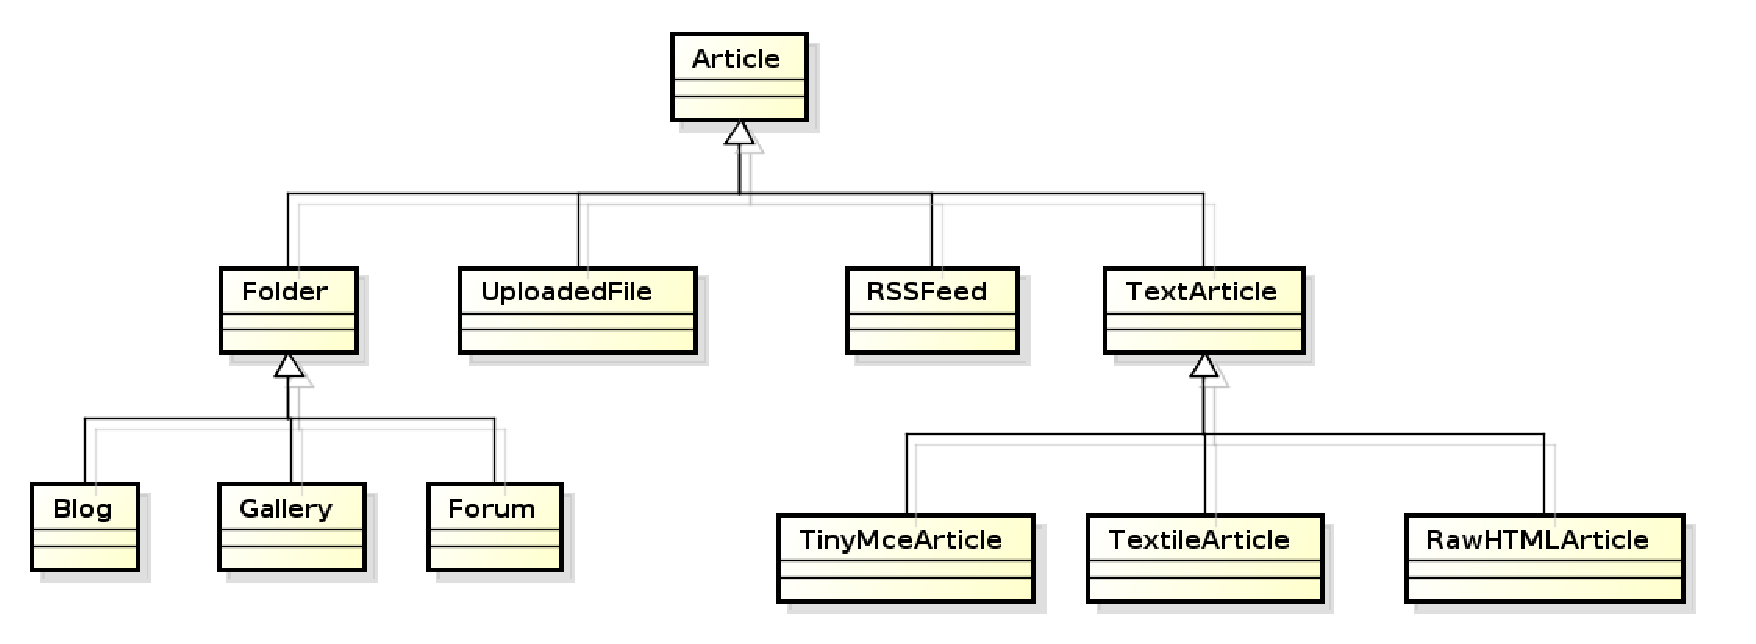
\includegraphics[keepaspectratio=true,scale=0.55]
      {figuras/domain_articles.eps}
    \caption{Entidades de domínio: tipos de artigos. Extraído de: \cite{bucher2013rede}}
    \label{domain_articles}
\end{figure}

Por fim, as entidades mostradas na Figura \ref{domain_articles} representam os principais tipos de conteúdos disponíveis no Noosfero, onde a classe \textbf{\textit{Article}}, ou Artigo, é uma especialização de todos os conteúdos disponíveis como: artigos de texto, pastas, blogs, galerias de imagens, fórum, arquivos e feeds de notícias.

O modelo de domínio aqui apresentado contempla o \textit{core} do noosfero. Para o acréscimo de melhorias e funcionalidades é necessário compreender a visão arquitetural dos \textit{plugins} d a plataforma, que será abordado na próxima seção.

\subsection{Plugins}
\label{plugins-noosfero}

Como é software em constante evolução, a arquitetura do Noosfero foi criada para ser altamente expansível, fazendo-se o uso de \textit{plugins}. Essa arquitetura permite que em cada ambiente fique a critério do usuário quais os \textit{plugins} ou novas funcionalidades serão habilitadas, o que torna o sistema flexível e modular.

% Aumentar figura 6
\begin{figure}[h]
    \centering
    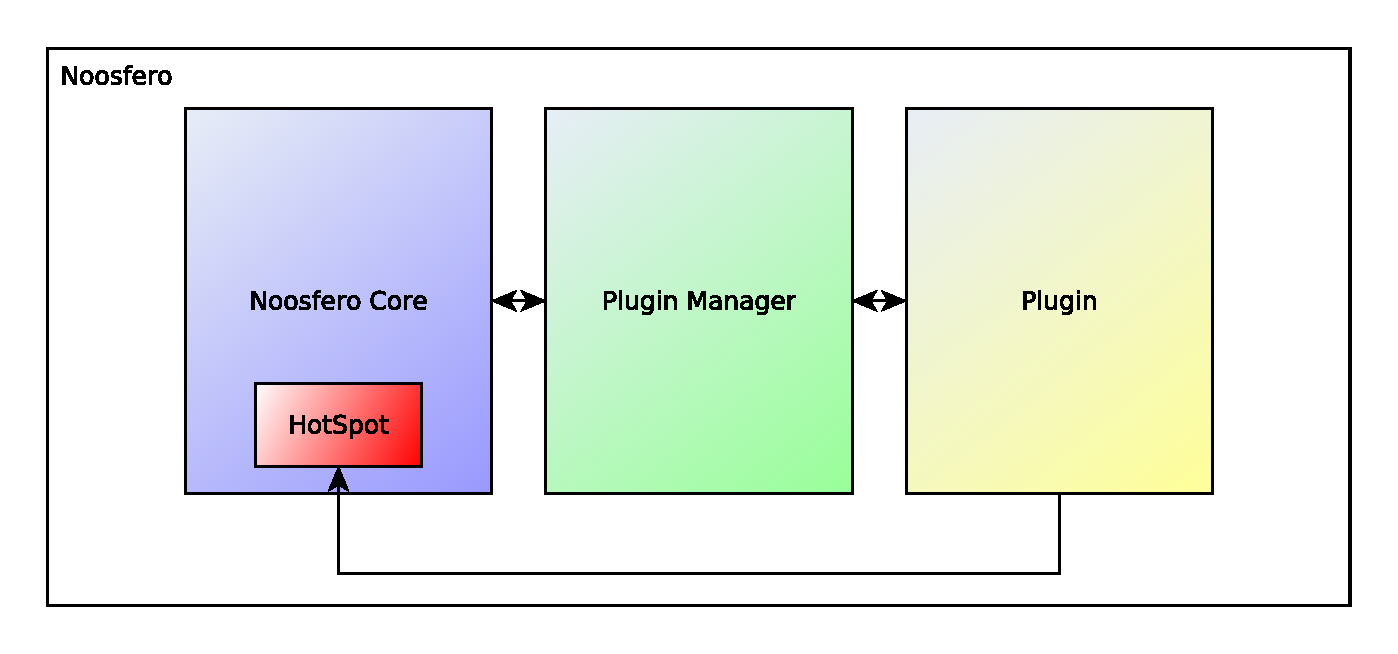
\includegraphics[keepaspectratio=true,scale=0.7]
      {figuras/estruturaDePlugins.eps}
    \caption{Estrutura de Plugins}
    \label{estrutura-plugins}
\end{figure}

A Figura \ref{estrutura-plugins} é uma abstração alto nível do funcionamento interno dos plugins no Noosfero. No \textit{core} do Noosfero temos os \textit{hotspots}, que são pontos de flexibilidade que permitem associar diferentes comportamentos na execução do sistema, permitindo a inserção de trechos de código e ou alteração de um determinado método sem comprometer suas funcionalidades básicas.

Os \textit{hotspots} são gerenciados por uma camada de abstração denominada \textit{Plugin Manager}, ou Gerenciador de \textit{Plugins}, que são chamadas pelo \textit{core} através de um metódo principal conhecido como \textit{dispatch}. Basicamente, o ciclo de execução pode ser descrito da seguinte maneira: durante a execução de alguma funcionalidade o método \textit{dispatch} é invocado por alguma funcionalildade do core, deste modo o gerenciador de plugins verifica todos os \textit{Plugins} que fazem uso daquele \textit{hotspot} e encaminha para cada um deles a execução de suas ações de acordo com sua implementação.

Essa arquitetura extensível adotada pelo Noosfero auxilia no controle da qualidade de código das novas funcionalidades. A camada de \textit{Plugins} localiza-se fora do código do seu núcleo, em uma pasta denominada \textit{plugins} em que desenvolvedor cria novas funcionalidades sem modificar o comportamento \textit{core} do Noosfero, fazendo uso dos \textit{dispatch}.

Adicionalmente como mencionado na Seção \ref{proc-desenvol-comunidade}, o Noosfero faz uso de testes para manter a integridade de seu código, desse modo esta prática é estendida aos \textit{plugins} que devem englobar seus respectivos testes para evitar a inserção de \textit{bugs} e mudanças inesperadas no comportamento do sistema. 

Assim sendo a evolução proposta para este trabalho será realizada através de plugins, como proposto na Seção \ref{desen-noosferAVA}

\section{Comunidade UnB}
\label{comunidade-unb}

A Comunidade.UnB é uma rede colaboração livre desenvolvida para que alunos, professores e servidores técnico-administrativos tenham um ambiente virtual de criação e compartilhamento de conhecimento colaborativo. É um ambiente virtual para o compartilhamento de ideias, produção de conteúdo colaborativo de modo que possam publicá-los para que possa ser de utilidade para outras pessoas ou parcelas da sociedade, uma vez que acredita-se que este é um dos papéis de uma Universidade \cite{bucher2013rede}.

\begin{figure}[!htb]
    \centering
    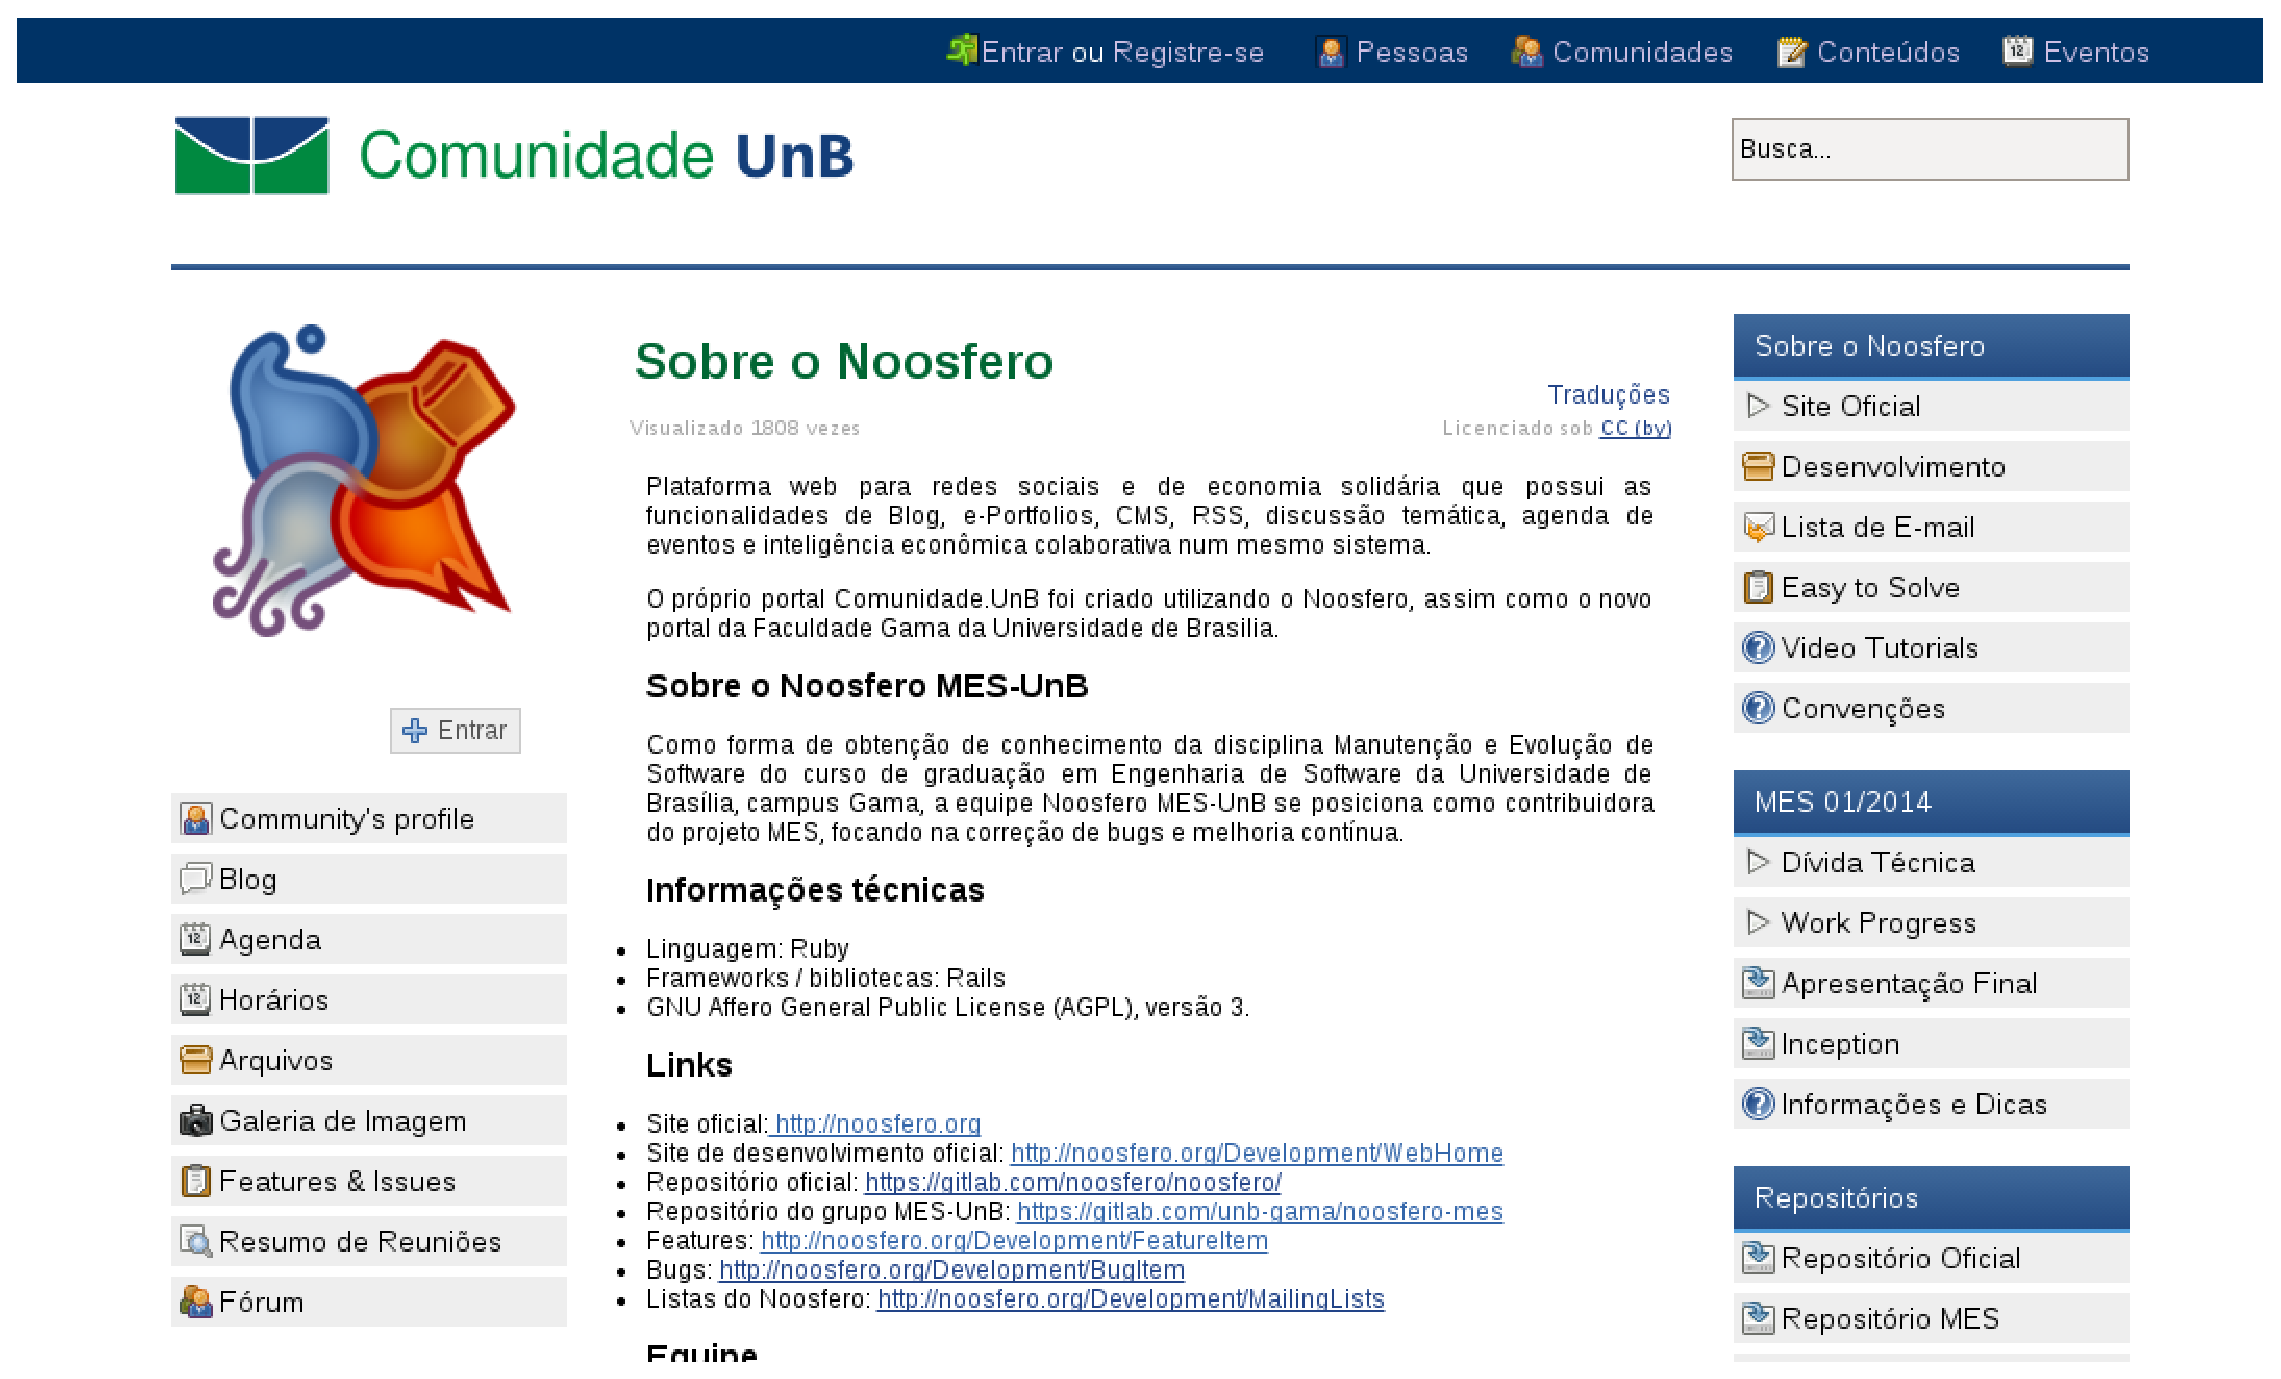
\includegraphics[keepaspectratio=true,scale=0.4]
      {figuras/comunidade-mes.eps}
    \caption{Exemplo do uso do Comunidade.UnB na disciplina de MES.}
    \label{comunidade-mes}
\end{figure}

Inspirada na rede social de colaboração Stoa \footnote{Disponível em: \url{https://social.stoa.usp.br/}}, da Universidade de São Paulo (USP), a Comunidade.UnB foi criada em 2013 a partir de um trabalho de conclusão de curso de Daniel Costa Bucher e até então está disponibilizada em ambiente de testes. Permite ao usuário a criação de seu espaço pessoal e a liberdade de publicar suas ideias, ou o conteúdo que desejar, por exemplo, na forma de blogs pessoais, blogs de disciplinas, pesquisas em andamento, dentre outras, além de compartilhar esse conteúdo para ser acessível para outros usuários dentro e fora da rede.

O Noosfero, descrito na Seção \ref{noosfero}, foi a plataforma utilizada para o desenvolvimento da Comunidade.UnB, por dispor de um grande potencial e devido às suas funcionalidades avançadas, que permitem a criação e o compartilhamento de conteúdo de forma satisfatória. Além de dispor de uma comunidade ativa e de posição geográfica favorável em relação ao seu núcle de desenvolvimento que se encontra no Brasil, facilitando a comunicação com os seus principais desenvolvedores.

Apesar da Comunidade.UnB estar disponibilizada como um ambiente de testes e não possuir uma vasta divulgação pela Universidade de Brasília, no seu primeiro ano de criação contava com 153 usuários e 14 comunidades. Ao final de maio de 2015 contabilizava 376 usuários e 30 comunidades demonstrando que houve crescimento.

Alguns professores adotaram a Comunidade.UnB como um ambiente de apoio ao Moodle, AVA oficial adotado pela UnB. Na Figura \ref{comunidade-mes} é apresentado um exemplo de seu uso na disciplina de Manutenção e Evolução de Software (MES) ministrada pelo professor Paulo Roberto Miranda Meirelles.

Esse é um exemplo de comunidade criada dentro do Comunidade.UnB, que possui características que se assemelham ao ambiente Moodle, como evidenciado na Seção \ref{comparacao-ava}, carece de alguns funcionalidades importantes mas com a vantagem da possibilidade de acesso do público ao conteúdo, e a continuidade do conteúdo desenvolvido por outras pessoas que eventualmente se juntem ao longo do tempo. Vale lembrar que em uma publicação de conteúdo os níveis de privacidade podem ser alterados basicamente entre públicos e privados.

As limitações da plataforma e a proposta de uso da Comunidade.UnB por professores para a criação de disciplinas, estimulam o desenvolvimento de funcionalidades que levem à plataforma Noosfero a assemelhar-se a um ambiente virtual de aprendizagem. 

Tendo como base todo o processo de desenvolvimento do Noosfero e as principais vantagens ao se utilizar o Comunidade.UnB, é o que nos motiva realizar a evolução da plataforma. Assim sendo é indispensável direcionar os esforços para a melhor satisfação dos usuários, o que nos leva a comparar no Capítulo \ref{metodologia} os recursos utilizados
nos AVA com o Noosfero e propor histórias a serem desenvolvidas.
